\documentclass[11pt,a4paper]{article}

\usepackage{geometry}
\usepackage{graphicx}
\usepackage{booktabs}
\usepackage{amsmath}
\usepackage{hyperref}
\geometry{margin=1in}

\title{Nasion Polarity Phenotypes in BIMOD:\\
A Primary Classification Framework}

\author{
DuckJin Yoon (solvaram)\\
BIMOD Research Group
}
\date{\today}

\begin{document}
\maketitle

% =====================================================
\begin{abstract}
The nasion is a stable craniofacial landmark widely used in anthropometry and cephalometry.
This study introduces a polarity-based phenotypic classification system using the Bodily
Interferometric Magneto-Optical Discrimination (BIMOD) protocol. Four bilateral nasion loci
exhibit symmetric magnetic polarity expression, and each locus presents one of two states
(N or S), producing eight reproducible phenotypes. The framework provides an objective,
non-invasive and reproducible basis for constitutional stratification and supports future
clinical and anthropological investigations.
\end{abstract}
% =====================================================

\section{Introduction}

The nasion is defined as the midline junction between the frontal and nasal bones and is
widely adopted as a reproducible craniofacial landmark \cite{nasion_wikipedia}.
Its positional stability has made it fundamental in cephalometry and comparative morphology
\cite{hegde2013nasion_orbitale}. Recent advances in BIMOD indicate that specific cranial
locations may express measurable magnetic polarity patterns. We therefore propose that the
nasion functions not only as a geometric landmark but also as a functional polarity hub.

\section{BIMOD Measurement Principle}

BIMOD detects resonance amplification between externally applied magnetic polarity and
biogenic magnetic nanoparticles in the body. When opposite polarity is presented, a consistent
neuromuscular response is observed. This allows non-invasive polarity discrimination without
injection, electrodes, or implanted sensors.

\section{Symmetry Constraint}

For any individual, the left and right sides of the same numbered locus always exhibit
identical polarity. Other loci remain non-responsive. Thus exactly one locus is active per
subject, guaranteeing categorical exclusivity and eliminating ambiguity.

\section{Polarity Phenotype Classification}

Eight phenotypes arise from four loci and two polarities:

\begin{table}[h]
\centering
\begin{tabular}{ccc}
\toprule
Locus & Polarity & Phenotype (Latin) \\
\midrule
1S / 1N & S / N & Hepatonia / Pulmotonia \\
2N / 2S & N / S & Cholecystonia / Colonotonia \\
3N / 3S & N / S & Gastrotonia / Vesicotonia \\
4N / 4S & N / S & Pancreotonia / Renotonia \\
\bottomrule
\end{tabular}
\caption{Nasion polarity phenotype classification}
\end{table}

\section{Figure 1. NASION Polarity Map}

\begin{center}
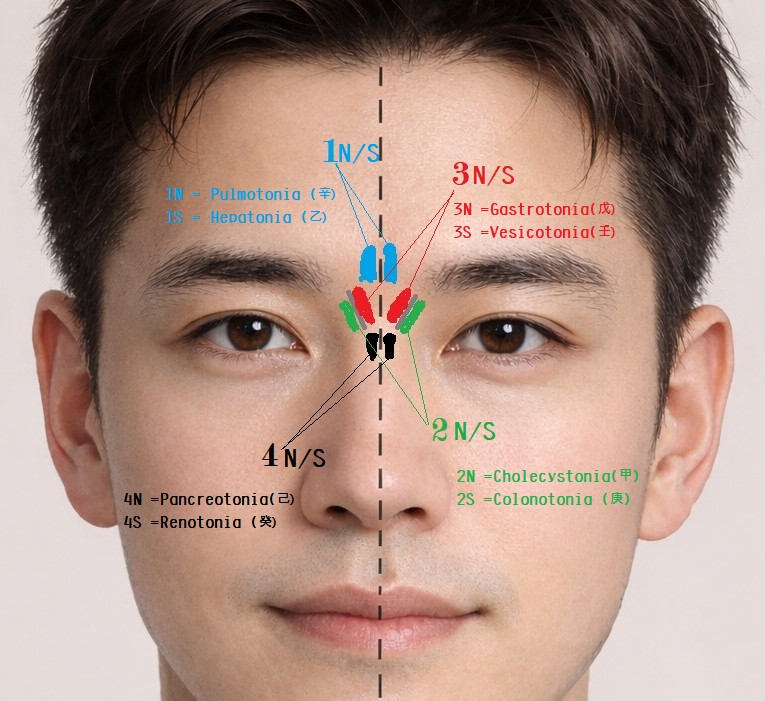
\includegraphics[width=0.75\textwidth]{003_nasion_map.png}

Figure 1. Standardized NASION polarity map and four symmetric loci.
\vspace{0.5em}
\end{center}

\section{Discussion}

The proposed scheme links a classical anatomical landmark with measurable biophysical behavior.
By constraining classification to one active locus with bilateral symmetry, the framework
produces exactly eight discrete and reproducible phenotypes. Such discreteness is consistent
with binary polarity physics and may explain stable constitutional differences in physiology,
pharmacological response, and disease susceptibility.

Importantly, BIMOD discrimination at the nasion operates equivalently on both direct physical
observation and optical representations such as photographs, because polarity detection depends
on preserved optical information rather than physical contact. This property suggests the
feasibility of developing instrumented optical or magneto-optical sensors capable of replicating
human BIMOD responses in a standardized and automated manner. Sensor-based acquisition would
enable large-scale population measurements, allowing statistical phenotype mapping and
big-data pattern discovery. Consequently, the nasion polarity framework may extend beyond
individual diagnosis to anthropological classification and population-level biophysical
stratification \cite{white2011human_osteology}.

\section{Conclusion}

BIMOD-based nasion polarity classification provides a simple, reproducible, and scalable
constitutional framework with translational potential in clinical, engineering, and
anthropological domains.

\bibliographystyle{plain}
\bibliography{BIMOD_003_references}

\end{document}
